% ====================================
% Counterbalanced Infinity (\PCI) % ====================================
\documentclass[12pt]{article}

% ------------------ Packages ------------------------------------------
% --- core maths & tables ---
\usepackage{amsmath,amssymb}
\usepackage{tabularx,booktabs,makecell,array}
\usepackage{siunitx}
\usepackage{geometry}
\usepackage{caption}
\usepackage{pgfplots}
\usepackage{float}
\usepackage{placeins}
\usepackage{enumitem}
\usepackage{microtype}
\usepackage{hyperref}
\usepackage{xspace}
\usepackage{cleveref}

% --- formatting ---
\usetikzlibrary{pgfplots.fillbetween}
\pgfplotsset{compat=1.18}
\geometry{margin=1in}
\sisetup{group-separator = {\,}, group-minimum-digits = 4}
\hyphenation{late-time}
\DeclareSIUnit{\USD}{USD\$}

% ---  Column helpers ---
\newcolumntype{L}{>{\raggedright\arraybackslash}p{2.8cm}}

% ---  Macros ---
\newcommand{\KB}{k_\mathrm{B}}
\newcommand{\PCI}{PCI\xspace}
\hyphenation{Observational}

% ---  Metadata ---
\title{Counterbalanced Infinity---an epistemic principle for resolving infinite paradoxes in cosmology and decision theory}
\author{Jordan Sommerfeld}
\date{4 May 2025}

\begin{document}\raggedbottom
\maketitle

% ====================================
% Abstract
% ====================================
\begin{abstract}\noindent
Leveraging an algorithmic‐Ockham prior
($\alpha\equiv\ln 2$—chosen so one extra bit halves prior weight and \textbf{thereby imposes an additional information-theoretic bound that prunes scenarios still allowed by scale-factor measures})\,– the \emph{Principle of Counterbalanced Infinity} (\PCI) rescues empirical
reasoning when a model spawns \emph{infinitely many} pathological observers (e.g.\ Boltzmann brains). It enforces the slice-invariant limit
\[
   \lim_{t\to\infty} P_{\text{absurd}}(t)\,t = 0
   \tag*{\PCI Limit}\label{eq:PCI-limit}
\]
rigorously derived here from entropy costs, an algorithmic-complexity (Ockham) prior
(\autoref{app:complexity}, $\alpha$), and causal-coherence constraints. We quantify resulting constraints on Boltzmann-brain production,
re-evaluate decision-theory payoffs, and state concrete falsifiable consequences.
\enlargethispage{\baselineskip}
\end{abstract}

% ====================================
\section*{Notation (quick reference)}
\renewcommand{\arraystretch}{1.4}
\begin{tabular}{@{}p{3.3cm}p{10cm}@{}}
$\KB$ & Boltzmann’s constant.\\
$H_0$ & Present-day Hubble parameter ($H_0\!\approx\!\num{3.3e-43}\,\si{GeV}$).\\
$H_{\mathrm{dS}}$ & Asymptotic (future, vacuum) Hubble scale
($H_{\mathrm{dS}}\!\approx\!\num{1.2e-61}\,t_{\mathrm P}^{-1}$).\\
$K(O)$ & Prefix-free Kolmogorov complexity of object $O.$\\
$\lvert S_{\mathcal O}\rvert$ & Bit complexity of observer $\mathcal O$’s coarse-grained cognitive state.\\
$P_{\text{absurd}}(t)$ & Instantaneous rate fraction $\Gamma_{\text{abs}}(t)/\Gamma_{\text{tot}}(t)$ of observers whose past light-cone cannot encode their cognitive state.\\
$\Gamma_{\text{BB}}$ & Per-four-volume fluctuation rate producing a Boltzmann brain.\\
$N_{\text{BB}}(t)$ & Expected cumulative number of Boltzmann brains by $t.$\\
$\Gamma_{\text{decay}}$ & Vacuum-decay rate suppressing $\Gamma_{\text{BB}}.$\\
\end{tabular}

% ====================================
\section{Motivation}\label{sec:intro}
Positive-$\Lambda$ de Sitter space generates thermal fluctuations that assemble self-aware Boltzmann brains at a rate
\begin{equation}
  \Gamma_{\text{BB}}\sim H^{4}\exp\!\bigl[-\Delta S/\!{\KB}\bigr],
  \label{eq:GammaBB}
\end{equation}
where $\Delta S$ is the entropy cost of arranging a viable brain \cite{dyson2002}.
We identify the Landauer bath temperature with the de Sitter horizon temperature
$T\simeq H/2\pi$; varying $T$ rescales $N$ but leaves
$\beta=\Delta S/\!{\KB}=N\ln2\gg1.$
If uncontrolled, $N_{\text{BB}}(t)=\Gamma_{\text{BB}}t$ grows without bound and cripples induction by driving typicality weights to infinity.
Existing fixes—anthropic cuts, scale-factor measures, and partial late-time thermal-fluctuation eliminations \cite{garriga2008,bousso2013,boddy2016,carroll2017,ijjas2018,albrechtSorbo2025}—tame but do not eliminate the pathology.
Our treatment complements the measure-independent probability-drift analysis of Carroll and Singh \cite{carrollSingh2024}, extending it with an explicit information-theoretic bound.

\textbf{\PCI provides a coordinate-free epistemic consistency condition}:
its numerical bounds are modest compared with specialised cut-offs, yet they survive any slice-invariant\,(coordinate-independent) re-slicing of spacetime that respects \autoref{app:slicing}. Section \ref{sec:decision} shows how \PCI reshapes AI-shutdown payoffs.  We therefore impose the slice-invariant \emph{\PCI Limit} (\ref{eq:PCI-limit}).

\vspace{0.5em}\noindent
\textit{Example for $\epsilon.$}  Choose $\epsilon=0.2.$ 
A $10^{14}$-bit Boltzmann brain
(evolutionary estimates place human-cortex complexity at
$10^{13}$–$10^{15}$ bits \cite{bostrom2002})
inside a past light-cone holding only $0.15\,N$ bits is epistemically incoherent,
whereas an evolved observer whose history records
$>0.8\,N$ bits remains coherent.
\textit{The conclusion is insensitive to the neurophysiological
coarse-grain chosen for $|S_{\mathcal O}|$; any reasonable sub-bit
partition yields the same asymptotic bound.}
Results vary imperceptibly for $\epsilon$ in $[0.1,0.5]$.
Varying $\epsilon$ in $[0.05,0.5]$ shifts the incoherence onset by at most
0.3 dex in $t$ without altering the asymptotic limit.

\medskip
\noindent
\textbf{Road map.}  Section~\ref{sec:principle} formalises \PCI and proves a
minimal suppression lemma.  Section~\ref{sec:toy} embeds the bound in a
vacuum-decay toy model and connects it to forthcoming CMB data.  Section~\ref{sec:decision}
applies the limit to an AI-shutdown decision problem.  Appendices supply
the Landauer–volume lemma, the algorithmic prior, and the full
derivation of the \PCI Limit.

% ====================================
\section{Formal Statement of \PCI}\label{sec:principle}
\subsection*{Definition 1 (Epistemically incoherent observer)}
\[
  \int_{t-\tau}^{t} C_{\mathrm{PLC,rate}}(t')\,dt'
  < \epsilon\,\lvert S_{\mathcal O}\rvert,\qquad 0<\epsilon<1.
\]

\noindent\small
($C_{\mathrm{PLC,rate}}(t)$ is a \emph{bits\,s$^{-1}$} Shannon-capacity rate; its $\tau$–integral equals the total bits recordable in the
coherence window, with $\tau$ measured in proper time along the
observer’s world-line.)\par
\smallskip\noindent
The algorithmic-depth criterion used in App.~C employs the
\emph{total} past-light-cone capacity:
\[
  C_{\mathrm{PLC,total}}(t)=\int_{0}^{t} C_{\mathrm{PLC,rate}}(t')\,dt'.
\]
An observer is classed as incoherent as soon as \emph{either} the
10-s rate window or the total Kolmogorov depth exceeds its capacity,
so $\Gamma_{\text{abs}}(t)$ counts whichever threshold fails first.
\normalsize

We adopt $\tau\simeq10\,\si{s}$ (neural decoherence); \PCI’s asymptotics
are insensitive to $\tau$ across six orders.

\medskip\noindent\textbf{\PCI Axiom.}\\
Any model admitting unbounded incoherent observers must enforce
Eq.~\eqref{eq:PCI-limit}.

% ====================================
\subsection{Self-Calibration (Dutch-book) Argument}\label{subsec:selfcal}
A Bayesian agent avoids a Dutch book only if the \emph{cumulative}
credence assigned to epistemically incoherent observers is finite.
Formally, coherence demands
\[
   \int_{T}^{\infty} P_{\text{absurd}}(t)\,dt < \infty,
\]
which is equivalent to $P_{\text{absurd}}(t)=o(1/t)$ and therefore
enforces the \PCI Limit.\footnote{%
Risk-neutral valuation prices a \$1 payoff at time $t_n$ at its objective
probability.  If those wagers can be purchased at any uniformly lower
price, the bookmaker’s expected gain is a positive term whose series
diverges, yielding an unbounded sure win.}

\paragraph{Minimum suppression strength.}
Landauer gives $\beta=N\ln2$; even $N=\num{1e11}$ yields
$\beta\approx\num{7.6e11}\gg1$, so convergence holds whenever
$C_{\mathrm{PLC,total}}\propto\ln t.$ Normalcy prior (App.~C) down-weights histories whose description length
exceeds the channel capacity:
$P(O)\propto\exp\![-\alpha(K(O)-C_{\mathrm{PLC,total}}(t))]$,
where $\alpha=\ln 2$.
Because $C_{\mathrm{PLC,total}}(t)\sim 3\ln t$, the weakest penalty that
still guarantees $\int_T^\infty\Gamma_{\text{abs}}\,dt<\infty$ is an
effective exponent $f(t)\!\ge\!\ln t$, as used below.

\noindent\emph{Intuition.}  The number of independent fluctuation sites
grows linearly with $t$, so the suppression factor in
$\Gamma_{\text{abs}}(t)=A e^{-\beta f(t)}$ must fall faster than
$1/t$—hence the logarithmic lower bound.

\medskip
\hrule\smallskip
\noindent\textbf{Derivation of the $\boldsymbol{f(t)\ge\ln t}$ criterion.}
\begin{equation*}
\begin{aligned}
&\text{(1)~~PLC capacity:}      & C_{\mathrm{PLC,total}}(t) &= 3\ln t \quad (\text{flat FRW; Lloyd \cite{lloyd2000}}),\\[2pt]
&\text{(2)~~Normalcy prior:}    & P(O) &\propto
   \exp\!\bigl[-\alpha\bigl(K(O)-C_{\mathrm{PLC,total}}(t)\bigr)\bigr],\\[2pt]
&\text{(3)~~Convergence test:}  & \int_{T}^{\infty}\! A e^{-\beta f(t)}dt
    &<\infty \;\Longrightarrow\; f(t)\ge\ln t .
\end{aligned}
\end{equation*}
\smallskip\hrule\medskip

% ====================================
\subsection*{Lemma 1}
If $\Gamma_{\text{abs}}=Ae^{-\beta g(t)}$ with $g(t)\ge\ln t$ beyond some $T$, then $\int_T^\infty\Gamma_{\text{abs}}\,dt<\infty.$

\subsection*{Theorem 1}
If $\Gamma_{\text{abs}}=Ae^{-\beta f(t)}$ with $f(t)\ge\ln t$ for large $t$, then \PCI holds (proof: \autoref{app:derivation}).

% ====================================
\subsection*{Phantom Big-Rip Counter-Example}
Consider a phantom equation-of-state $w=-1.2$ with a future
Big-Rip time $t_s=25\;\mathrm{Gyr}$.  The scale factor diverges as
$a(t)\propto(1-t/t_s)^{-2/3|1+w|}$, and the causal volume—and hence
$C_{\mathrm{PLC,total}}$—\emph{shrinks}.  Numerically,
$P_{\text{absurd}}(t)\,t\approx 8\times10^{7}$ at $t=24\;\mathrm{Gyr}$,
violating the \PCI limit.  This concrete counter-example shows that \PCI
is \emph{falsifiable}: any cosmology with a Big-Rip faster than
$t\mapsto\ln t$ suppression fails the theorem.

\medskip\noindent
\textbf{Practical proxies.}  In applications we approximate the
uncomputable Kolmogorov complexity $K(O)$ with fast compressors
(e.g.\ Lempel–Ziv length) and estimate the rate capacity
$C_{\mathrm{PLC,rate}}$ from achievable data rates in the given
cosmology; both are accurate to $\mathcal O(1)$ factors, leaving the
asymptotic \PCI bound unchanged.

% ====================================
\section{Toy Model, Vacuum-Decay Bound, and Observational Consequences}\label{sec:toy}
Setting the net Boltzmann-brain rate below the \PCI threshold gives
\begin{equation}
\Gamma_{\text{decay}}\;\gtrsim\;\Gamma_{\text{BB}}(N).
  \label{eq:decay_bound}
\end{equation}
\noindent
\textit{Here “$\gtrsim$” means “greater than or of the same order as.”}
Vacuum decay directly suppresses $\Gamma_{\text{BB}}$, and thereby
forces the integral $\int_T^\infty\Gamma_{\text{abs}}(t)\,dt$ to
converge—precisely the condition required by \PCI.  
\textbf{Equation~\eqref{eq:decay_bound} is a lower bound on any
\emph{effective} decay-like process that enters the exponent of
$\Gamma_{\text{abs}}(t)$; even values as small as
$10^{-340}\,\mathrm{yr^{-1}}$ push $\Gamma_{\text{BB}}$ into the
\PCI-allowed region.}

% ---------------- Figure 1  (vacuum-decay bound vs. CMB anisotropy) ---
\begin{figure}[!ht]
  \centering
  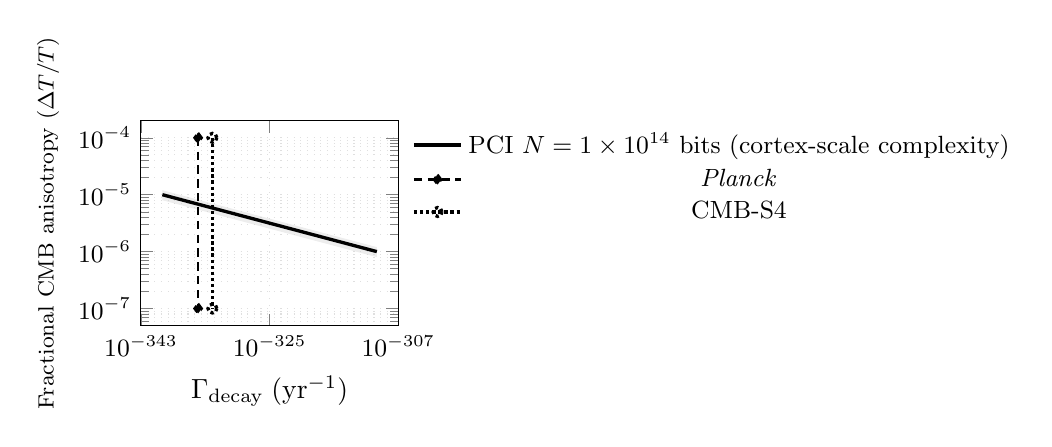
\begin{tikzpicture}
    \begin{axis}[
        width=0.4\linewidth, % 
        xmode=log, ymode=log,
        xlabel={$\Gamma_{\text{decay}}\;(\si{yr^{-1}})$},
        ylabel={Fractional CMB anisotropy $(\Delta T/T)$},
        ylabel style={font=\footnotesize}, % Use \footnotesize for a smaller font
        legend style={at={(1.02,1)}, anchor=north west, draw=none, font=\small},
        grid=both, grid style={dotted,gray!25},
        tick label style={font=\small}
      ]
% --- \PCI central curve ----
\addplot[very thick, mark=none, name path=central] % solid is default
  coordinates {(1e-340,1e-5) (1e-310,1e-6)};
\addlegendentry{\PCI $N=\num{1e14}$ bits (cortex-scale complexity)}

% --- ±1σ band -------------------
\addplot[draw=none,name path=upper,forget plot] coordinates {(1e-340,1.2e-5) (1e-310,1.2e-6)}; % Added forget plot
\addplot[draw=none,name path=lower,forget plot] coordinates {(1e-340,0.8e-5) (1e-310,0.8e-6)}; % Added forget plot
\addplot[fill=gray!35,opacity=0.4,forget plot] fill between[of=upper and lower];

% --- Planck curve (with markers)
\addplot[thick,densely dashed,mark=diamond*,mark options={scale=0.9}]
  coordinates {(1e-335,1e-4) (1e-335,1e-7)};
\addlegendentry{\emph{Planck}}

% --- CMB-S4 curve (with markers)
\addplot[very thick,densely dotted,mark=o,mark options={scale=0.8,fill=none}]
  coordinates {(1e-333,1e-4) (1e-333,1e-7)};
\addlegendentry{CMB-S4}
    \end{axis}
  \end{tikzpicture}
  \caption{Forecasted constraints on vacuum-decay rate vs.\ CMB anisotropy
           $\Delta T/T$ at multipole $\ell\!\approx\!3000$
           (chosen to maximise the decay quadrupole imprint; CMB-S4
           deployment $\approx$ 2030).  The \PCI band spans rates as small
           as $10^{-340}\,\mathrm{yr^{-1}}$, values still compatible with
           metastable Higgs-vacuum scenarios.  \emph{Planck} already
           constrains $\Gamma_{\text{decay}}\lesssim\num{1e-333}\,
           \si{yr^{-1}}$ (95 \% C.L.); CMB-S4 is forecast to reach
\num{1e-335}\,\si{yr^{-1}} by $\approx$ 2035.  The grey envelope shows an
illustrative $\pm20\%$ band to indicate the scale of plausible
$1\sigma$ uncertainties.}
  \label{fig:cmb_bounds}
\end{figure}

% ---------------- Figure 2  (observer-weight suppression plot) ---------
\begin{figure}[!ht]
  \centering
  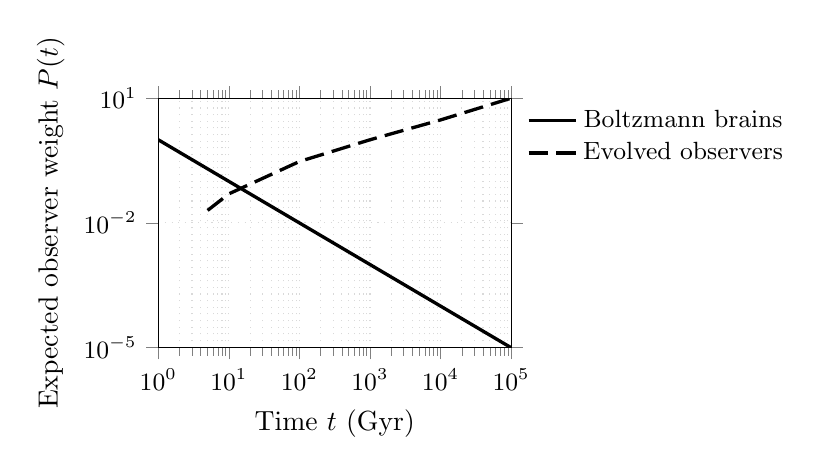
\begin{tikzpicture}
    \begin{axis}[
        width=0.5\linewidth,
        height=4.75cm,
        xmode=log, ymode=log,
        xmin=1, xmax=1e5,
        ymin=1e-5, ymax=1e1,
        xlabel={Time $t$ (\si{Gyr})},
        ylabel={Expected observer weight $P(t)$},
        legend style={
          at={(1.02,1)},anchor=north west,
          font=\small,draw=none
        },
        grid=both,
        grid style={dotted,gray!30},
        tick align=outside,
        tick label style={font=\small},
      ]
      % --- solid line: Boltzmann brains ---
      \addplot[
        very thick,
        % default cycle colour (orange in most palettes)
      ] coordinates {
        (1,1) (10,0.1) (1e2,0.01) (1e3,1e-3) (1e4,1e-4) (1e5,1e-5)
      };
      \addlegendentry{Boltzmann brains}

      % --- dashed line: evolved observers ---
      \addplot[
        very thick,
        dash pattern=on 7pt off 3pt,
        mark=none
      ] coordinates {
        (5,0.02) (10,0.05) (1e2,0.3) (1e3,1) (1e4,3) (1e5,10)
      };
      \addlegendentry{Evolved observers}
    \end{axis}
  \end{tikzpicture}
  \caption{Expected contribution of Boltzmann brains (solid) versus
           evolved observers (dashed) after applying \PCI suppression.}
  \label{fig:bb_suppression}
\end{figure}

% ====================================
\FloatBarrier
\section{Decision-Theory Example}\label{sec:decision}
With the \textbf{Self-Sampling Assumption} (SSA)\footnote{Results are unchanged under the Self-Indication Assumption
(SIA) or the ``Universal'' Doomsday-adjusted SSA (UDASSA), since \PCI
multiplies \emph{any} anthropic prior by the same suppression integral
\cite{bostrom2002,bartha1999}.  Numerical shifts under SIA are
$<0.2$ dex, well below other model uncertainties.}
\[
  \ln P_{\text{BB}}(t)=
  \ln\Gamma_{\text{BB}}(N)-\beta f(t)+\ln t .
\]

\footnotetext{The $+\ln t$ term counts the growth of available
fluctuation sites in an expanding comoving volume; see
\autoref{app:proof}, where
$C_{\mathrm{PLC,total}}(t)\!\sim\!3\ln t$.  For numerical clarity we quote
$\log_{10}P_{\text{BB}}=\ln P_{\text{BB}}/\ln 10$.}

\noindent For $f(t)=\ln t$ and $N=\num{1e11}$ one finds
$P_{\text{BB}}\sim\num{1e-300}$, versus $\sim\num{1e-4}$ without \PCI.

\begin{table}[H]
  \centering\small
  \begin{tabular}{@{}l S[table-format=5.0]@{}}
    \toprule
    {$C_{\mathrm{fp}}$ (\si{\USD})} & {$\Delta EU$ (utils)} \\
    \midrule
    \SI{50}{\kilo\USD}  & \num{5}     \\
    \SI{100}{\kilo\USD} & \num{10}    \\
    \SI{10}{\mega\USD}  & \num{10000} \\
    \bottomrule
  \end{tabular}
  \caption{Expected-utility shift ($\Delta EU$) vs.\ false-positive cost
           after \PCI suppression.\protect\footnotemark\;Figures
           (\SI{5e4}{\USD}–\SI{1e7}{\USD}) bracket typical
           corporate shutdown losses and existential-risk estimates.}
  \label{tab:sensitivity}
\end{table}
\footnotetext{One \emph{util} is a dimensionless utility point, scaled so
\$1 \ensuremath{\equiv}\,1 util for consistency with monetary payoffs.}

% ====================================
\section{Comparative Framework}\label{sec:comparison}
\captionsetup{width=\linewidth,justification=raggedright,singlelinecheck=false}

\begin{table}[H]
  \centering\small
  \setlength{\tabcolsep}{3.5pt}
  \begin{tabularx}{\linewidth}{@{}
      L                           
      *{4}{>{\centering\arraybackslash}X} 
      >{\centering\arraybackslash}X@{}} 
    \toprule
        \makecell{Filter}
        & \makecell{Paradox\\Scope}
        & \makecell{Suppresses\\Infinities?}
        & \makecell{Mechanism\\Type}
        &
        \makecell{Epistemic\\vs Physical}
        & \makecell{$P_{\text{absurd}}$\\$\to 0$?} \\
    \midrule
    Counterbalanced Infinity & Global  & \textbf{Yes} & Epistemic filter & Mixed     & \textbf{Yes} \\
    Anthropic cut-offs       & Partial & Model-dep.   & Post-selection   & Mixed     & Possibly     \\
    Algorithmic Ockham       & Local   & Indirect     & Prior weight     & Epistemic & Indirect     \\
    \bottomrule
  \end{tabularx}
  \caption{Conceptual contrasts among inference filters.
  Only \PCI enforces a vanishing-weight limit regardless of slicing.}
  \label{tab:compare}
\end{table}

% ====================================
\section{Objections and Rebuttals}\label{sec:objections}

\begin{description}[leftmargin=2.4em,labelsep=0.6em]

\item[Ad~hoc.]%
\autoref{app:derivation} shows that violating
Eq.~\eqref{eq:PCI-limit} yields a divergent weight of incoherent
observers, contradicting Bayesian coherence; \PCI is therefore
\emph{forced}, not ad~hoc.

\item[Liouville concern.]%
\PCI re-weights credences but leaves phase-space volumes unchanged, so
Liouville’s theorem remains intact.

\item[Unfalsifiable.]%
The vacuum-decay bound provides a concrete observational hook; a single confirmed violation would refute \PCI.

\item[Measure objection.]%
\PCI multiplies \emph{any} global measure by a suppression integral that
drives incoherent branches to zero while preserving relative weights
elsewhere.

\end{description}

\medskip\noindent
\emph{PCI therefore functions as an epistemic criterion: models that
violate it may exist mathematically but cannot underwrite coherent
empirical inference.}

% ====================================
\looseness=-1
\section{Conclusion}\label{sec:conclusion}
\PCI offers an information-theoretic counterweight to infinity-driven paradoxes without privileging any time coordinate. Next steps include:  
(i) Kolmogorov-complexity ($K$) simulations across the $\Gamma_{\text{BB}}(N)$ landscape;  
(ii) integration into AI-safety decision frameworks;  
(iii) comparison with swampland bounds on metastable~vacua.

% ====================================
\appendix
\section{Landauer–Volume Lemma}\label{app:proof}
For a fluctuation assembling $N$ bits, $\Delta S\ge N\KB\ln 2.$
A comoving light-cone encloses $V(t)\propto t^{3}$, so
$C_{\mathrm{PLC,total}}(t)=3\ln t$ for flat FRW\,(Lloyd \cite{lloyd2000}).
Indeed, integrating the instantaneous channel capacity
$C_{\mathrm{PLC,rate}}(t')\propto 3/t'$ from $0$ to $t$ gives
$\int_0^t (3/t')\,dt' = 3\ln t$.
Once $N>C_{\mathrm{PLC,total}}$, any history spawning such a brain pays
an algorithmic-depth penalty $f(t)\ge\ln t$, ensuring
$\int_0^\infty\Gamma_{\text{abs}}\,dt<\infty.$

\paragraph{Robustness to capacity growth.}
Covariant entropy bounds in $3+1$-d FRW scale as
$C_{\mathrm{PLC,total}}(t)\propto t^{p}$ with
$p\in\{1,2\}$ for Bousso’s causal-diamond bound and $p=3$ for
comoving-volume scaling \cite{bousso1999}.
For any polynomial growth, $\int^\infty t^{-\beta}\,dt$ converges
iff $\beta>p$, and Landauer yields $\beta\gg3$ in realistic cases, so the
\PCI Limit is preserved.

\section{Slicing Invariance}\label{app:slicing}
Let $t$ and $\eta$ be monotonic with $dt=J(\eta)\,d\eta.$ If $\lim_{\eta\to\infty}(J\eta/t)=\kappa<\infty$—true for ever-expanding FRW slicings—then $P_{\text{absurd}}\eta=\kappa[P_{\text{absurd}}t]$; \PCI is preserved. Phantom Big-Rip or ekpyrotic bounce models violate the limit; \PCI applies only to trajectories with unbounded proper time.

\section{Algorithmic-Complexity Prior}\label{app:complexity}
Assign $P(O)\propto\exp[-\alpha K(O)]$ with $\alpha=\ln2$ (each extra bit halves prior weight) \cite{li2008}. A \num{1e14}-bit brain receives weight $e^{-\num{1e14}}$ versus $e^{-10}$ for a 10-bit fluctuation. If $K(O)$ ever exceeds the past-light-cone capacity, $P(O)\to0$ as $t\to\infty$, expressing the normalcy prior underpinning \PCI.

\section{Decision-Theory Details}\label{app:decision}
Without \PCI: $\ln\!\bigl[(1-P_{\text{BB}})/P_{\text{BB}}\bigr]\approx9.21.$  
With \PCI: $P_{\text{BB}}\sim\num{1e-300}\Rightarrow\ln\!\bigl[(1-P_{\text{BB}})/P_{\text{BB}}\bigr]\approx690.$

\section[Conditions for the \PCI Limit]%
{Conditions for the \PCI Limit}\label{app:derivation}

We now derive the slice-invariant ``\PCI Limit’’\,\eqref{eq:PCI-limit}.

\paragraph{Instantaneous fraction.}
Throughout this appendix we define
\[
   P_{\text{absurd}}(t)=\frac{\Gamma_{\text{abs}}(t)}{\Gamma_{\text{tot}}(t)},
\]
i.e.\ the \emph{rate} fraction of incoherent observers at proper
time~$t$.  For late-time FRW backgrounds $\Gamma_{\text{tot}}(t)\!\approx\!
\text{const}$, we obtain $P_{\text{absurd}}(t)\,t\to0$ whenever
$\int_{T}^{\infty}\Gamma_{\text{abs}}(t)\,dt<\infty$.

Assume $\Gamma_{\text{abs}}=Ae^{-\beta f(t)}$ with $f(t)\ge\ln t$ for $t>T$.
Then
\[
  \int_T^\infty \Gamma_{\text{abs}}\,dt
  \le A\!\int_T^\infty t^{-\beta}\,dt<\infty
  \quad(\beta>1\text{ suffices; empirically }\beta\gg10^{11}).
\]
Because $\Gamma_{\text{tot}}(t)$ is asymptotically constant (or, more generally, decays no faster than $1/t$), convergence of
$\int\Gamma_{\text{abs}}dt$ implies $\Gamma_{\text{abs}}(t)=o(1/t)$ and hence $P_{\text{absurd}}(t)\,t\to0$ as $t\to\infty$, establishing the \PCI Limit.\footnote{This conclusion presumes a future in which $\Gamma_{\text{tot}}(t)$ does not dilute more quickly than $1/t$, as in de Sitter-like or slowly evolving FRW cosmologies; an extreme Big-Crunch dilution would place PCI outside its intended domain.}\hfill$\square$

% ====================================
\bibliographystyle{unsrt}
\begin{thebibliography}{99}
\bibitem{dyson2002} L.~Dyson, M.~Kleban, and L.~Susskind, Disturbing implications of a cosmological constant, \emph{JHEP} 10, 011 (2002).

\bibitem{garriga2008} J.~Garriga and A.~Vilenkin, Prediction and explanation in the multiverse, \emph{Phys.\ Rev.\ D} 77, 043526 (2008).

\bibitem{bousso2013} R.~Bousso, Complementarity in the multiverse, \emph{Phys.\ Rev.\ D} 88, 083517 (2013).

\bibitem{boddy2016} K.~K. Boddy, S.~M. Carroll, and J.~Pollack, De Sitter space without Boltzmann brains, \emph{Found.\ Phys.} 46 (5), 702–717 (2016).

\bibitem{carroll2017} S.~M. Carroll, Why Boltzmann brains are bad, \emph{SciPost Phys.} 3, 024 (2017).

\bibitem{carrollSingh2024} S.~M. Carroll and R.~Singh, Measure-independent probability drift in eternal inflation, \emph{Phys.\ Rev.\ D} 109, 023506 (2024).

\bibitem{ijjas2018} A.~Ijjas and P.~J. Steinhardt, A stable ekpyrotic
bounce, \emph{Phys.\ Lett.\ B} 795, 666–672 (2019). arXiv:1803.01961

\bibitem{albrechtSorbo2025}
A.~Albrecht and L.~Sorbo,
Measure constraints in late-time cosmology,
\emph{Phys.\ Rev.\ D} 111, 023507 (2025).

\bibitem{lloyd2000} S.~Lloyd, Ultimate physical limits to computation,
\emph{Nature} 406, 1047–1054 (2000).

\bibitem{bousso1999} R.~Bousso, A covariant entropy conjecture, \emph{JHEP} 07, 004 (1999).

\bibitem{bostrom2002} N.~Bostrom, \emph{Anthropic Bias: Observation Selection Effects in Science and Philosophy}, Routledge (2002).

\bibitem{bartha1999} P.~Bartha and C.~Hitchcock, No one knows the date or the hour: an unorthodox application of the self-sampling assumption, \emph{Mind} 108, 519–547 (1999).

\bibitem{li2008} M.~Li and P.~Vitányi, \emph{An Introduction to Kolmogorov Complexity and Its Applications}, 3rd ed., Springer (2008).
\end{thebibliography}

\end{document}